\documentclass[a4paper,article,10pt]{article}

%-- pacotes --------------------------------------------------------------------
\usepackage[brazil]{babel}
\usepackage[utf8]{inputenc}
\usepackage[active]{srcltx}

\usepackage{latexsym,amsmath,amssymb,amsfonts,amsthm}
\usepackage{url}
\usepackage{graphicx,color}
\usepackage{indentfirst}
\usepackage[portugues,boxed,vlined,linesnumbered]{algorithm2e}
\usepackage{ifthen}
\usepackage[T1]{fontenc}
\usepackage{gastex}
\usepackage{booktabs}

\usepackage[round,comma,longnamesfirst]{natbib}

%-- comandos -------------------------------------------------------------------
\renewcommand{\familydefault}{\sfdefault}
\renewcommand{\thefootnote}{\fnsymbol{footnote}}
\newtheorem{thm}{Teorema}[section]
\newcommand{\resumo}[1]{
  \begin{abstract}
    {\rm #1}
  \end{abstract}
}

\newcommand{\implica}{\Rightarrow}
\newcommand{\sse}{\text{ se e somente se }}
\newcommand{\talque}{\,|\,\,}
\newcommand{\Equiv}{\sim}

\newcommand{\nao}{\textsf{ não }}
\newcommand{\ou}{\textsf{ ou }}
\newcommand{\e}{\textsf{ e }}
\newcommand{\se}{\textsf{ se }}
\newcommand{\entao}{\textsf{ então }}
\newcommand{\paratodo}{\textsf{ para todo }}
\newcommand{\paralgum}{\textsf{ para algum }}

\newcommand{\bN}{\mathbb{N}}
\newcommand{\bQ}{\mathbb{Q}}
\newcommand{\bR}{\mathbb{R}}
\newcommand{\bZ}{\mathbb{Z}}
\newcommand{\bC}{\mathbb{C}}
\newcommand{\bE}{\mathbb{E}}
\newcommand{\bP}{\mathbb{P}}

\newcommand{\cA}{\mathcal{A}}
\newcommand{\cB}{\mathcal{B}}
\newcommand{\cC}{\mathcal{C}}
\newcommand{\cD}{\mathcal{D}}
\newcommand{\cE}{\mathcal{E}}
\newcommand{\cF}{\mathcal{F}}
\newcommand{\cI}{\mathcal{I}}
\newcommand{\cJ}{\mathcal{J}}
\newcommand{\cP}{\mathcal{P}}
\newcommand{\cR}{\mathcal{R}}
\newcommand{\cS}{\mathcal{S}}
\newcommand{\cT}{\mathcal{T}}

\newcommand{\chaves}[1] {{\left \{ {#1} \right \}}}
\newcommand{\colchetes}[1] {\left [ {#1} \right ]}
\newcommand{\parenteses}[1] {\left ( {#1} \right )}
\newcommand{\barras}[1] {\left | {#1} \right |}
\newcommand{\floor}[1] {\left \lfloor {#1} \right \rfloor}
\newcommand{\ceil}[1] {\left \lceil {#1} \right \rceil}
\newcommand{\floorfrac}[2] {\floor{\frac{#1}{#2}}}
\newcommand{\ceilfrac}[2] {\ceil{\frac{#1}{#2}}}
\newcommand{\Max}[1] {\max\chaves{#1}}
\newcommand{\Min}[1] {\min\chaves{#1}}
\newcommand{\Exp}[1]{\EE\colchetes{#1}}
\newcommand{\Prob}[1]{\PP\parenteses{#1}}

%-- título ---------------------------------------------------------------------
\title{{\Huge Paralelização do problema de Arbitragem}}
\author{\small Cássio Jandir Pagnoncelli\footnote{cjp07@inf.ufpr.br}
   \and \small Gabriel Augusto Sobral\footnote{gags07@inf.ufpr.br}}
\date{\scriptsize \today}

%-- documento ------------------------------------------------------------------
\begin{document}
%\flushbottom
\maketitle
%\tableofcontents

  % abstração
  \begin{abstract}
    \scriptsize
    Esse é um relatório apresentado para a disciplina de Programação Paralela,
    CI-316, ministrada pelo professor Dr. Fabiano Silva na Universidade Federal
    do Paraná em 2011/1 pelos alunos Cássio Jandir Pagnoncelli e Gabriel Augusto
    Sobral, ambos da graduação em Bacharelado em Ciência da Computação.
  \end{abstract}

  \section{Prolema}

    Seja $K_n = (V,E)$ um dígrafo completo de $n$ vértices cujos pesos das
    arestas, uma para cada par de vértices distintos, formam o conjunto $E$.
    Um caminho é uma sequência de vértices de $V$ que não contém ciclo, i.e. não
    há repetição de vértices no caminho; assim, um caminho de $v_{inicio}$ até
    $v_{fim}$ ($v_{fim} \ne v_{inicio}$) é uma sequência
    \begin{equation*}
      (v_{inicio} = v_1, v_2, \cdots, v_{k-1}, v_k = v_{fim})
    \end{equation*}
    satisfazendo $i\ne j \implica v_i \ne v_j$ no caminho.

    Diferentemente da noção usual de custo de caminho, definiremos o custo de um
    caminho $c = \chaves{v_i}_{i=inicio}^{fim}$, $custo(c)$, por
    \begin{equation*}
      \prod_{i=inicio}^{fim-1} peso(v_i, v_{i+1});
    \end{equation*}
    isto é, o produto dos pesos das arestas no caminho. 
    Um desses caminhos tem custo mínimo, que é de nosso interesse, que
    chamaremos de caminho mínimo.
    (Repare que no nosso dígrafo o caminho mínimo de $u\in V$ até $v\in V$ não é
    necessariamente o caminho de custo mínimo de $v$ até $u$.)

    O problema computacional que iremos paralelizar é
    \begin{description}
    \item [Instância:] Um dígrafo completo $K_n$ com $n\geq 2$ vértices.
    \item [Resposta:] Uma tabela de dimensões $n$ x $n$ com $2\,\binom{n}{2}$
      elementos\footnote{Uma tabela completa, exceto pelos elementos da diagonal
      principal, que representam a inexistência de uma aresta com origem e
      destino num mesmo vértice.}, cada célula $(lin,col)$, com $lin\ne col$,
      contendo o caminho de menor custo com origem no vértice indexado por
      `$lin$' e com destino no vértice indexado por `$col$'.
    \end{description}

    A representação do problema está descrita no arquivo `LEIAME', que acompanha
    o pacote contendo o código-fonte do programa.

  \section{Algoritmo sequencial e sua análise}
    
    Pela natureza desse problema, especialmente pelo modo como foi definido o
    custo de um caminho, esse problema se torna inerentemente difícil de ser
    resolvido, conforme veremos a seguir.

    Não é nada intuitivo um modo de fazer podas nas subárvores que buscam todas
    as permutações de caminhos; por isso não é nada claro usar técnicas de
    branch-and-bound que sejam eficientes, já que todas as permutações deverão
    ser percorridas.
    Tudo isso porque não há nenhuma garantia de que aumentando um dado caminho
    em um vértice o custo desse caminho pode diminuir.

    O algoritmo\footnote{A chamada inicial desse algoritmo é feita com $k=1$,
      $V:= [v_1, \cdots, v_n]$ (onde os vértices $v_i$ ($1 \leq i \leq n$)
      formam $V(K_n)$) e uma tabela $T$ inicialmente valorada com cada célula
      sendo  um caminho nulo de custo infinito.} faz uma busca exaustiva usando
    backtracking  sobre o dígrafo buscando menores caminhos para cada par de
    vértices distintos, atualizando uma tabela contendo os caminhos de menores
    custos para cada um dos $n^2-n$ pares de vértices distintos.
    O ``core'' desse algoritmo que faz backtracking é:

    \begin{algorithm}[H]
      \caption{\sc Backtracking}

      \SetKwBlock{Begin}{inicio}{fim}
      \SetKw{Retorna}{devolva}
      
      \Entrada{
        \begin{enumerate}
        \item um inteiro positivo $k$;
        \item um vetor $V$ indexado de $1$ a $n=|V|$;
        \item uma tabela $T[1 \ldots n][1 \ldots n]$, cada célula sendo um
          caminho.
        \end{enumerate}
      }
      \Saida{A tabela $T$ preenchida em todas as células, exceto naquelas
        da diagonal principal.}

      \Begin{
          \Se{$custo\_caminho(V\colchetes{1 .. inicio}) < 
            custo\_caminho(T[V[1]][V[inicio]])$}{
            $T[V[1]][V[inicio]] ~ \leftarrow ~ V\colchetes{1..inicio}$ \;
            }
          
          \ParaCada{$i \in [inicio..n]$}{
            $\textsc{troca}(V[inicio], V[n])$ \;
            $T ~ \leftarrow ~ \textsc{Backtracking}(inicio + 1, V, T)$ \;
            $\textsc{troca}(V[inicio], V[n])$ \;
          }

          \Retorna{$T$} \;
      }
    \end{algorithm}
    onde $\textsc{troca}(V[i], V[j])$ troca os valores de $V[i]$ e $V[j]$.

    O melhor e o pior caso desse algoritmo são superior e inferiormente
    limitados pela mesma função que descreve o tempo de execução para uma dada
    instância; essa dificuldade de não encontrar nenhuma solução óbvia, numa
    primeira aproximação ao problema, nos serviu de motivação para recorrer ao
    paralelismo na intenção de obtermos respostas tão próximas quanto possível
    do utópico tempo $t_S (n)/p$, i.e. resposta na $p$-ésima parte de
    tempo da versão sequencial, onde $p$ é o numero de processadores executando
    o algoritmo em paralelo.

    Dado como entrada do programa que implementa o algoritmo acima, na versão
    sequencial, o dígrafo completo $K_n$ com $n\geq 2$ vértices, todas as
    permutações de tamanhos de pelo menos $2$ de todos os vértices somam
    $\sum_{k=2}^n k!$, que não excedem a quantidade de $(n+1)!$.

    Levando em conta que a entrada é uma matriz de adjacências de um dígrafo de
    $n$ vértices; isto é, uma entrada de tamanho $1 + 2\,\binom{n}{2}$, conforme
    a representação da entrada já comentada.
    A saída do algoritmo é uma tabela de dimensões $n$ x $n$ com
    $2\,\binom{n}{2} = n^2 - n$ elementos, também já comentada.
    Logo, o tempo de execução do algoritmo sequencial com entrada $X$ (um
    dígrafo de $n$ vértices), $t_S(X)$, é
    \begin{align*}
      t_S(X) &= t_{\textsc{leitura}}(X) + t_{\textsc{backtracking}}(X)
                + t_{\textsc{saida}}(X) \\
             &= \parenteses{1 + 2\,\binom{n}{2}} + \parenteses{\sum_{k=2}^n k!}
                + \parenteses{2\,\binom{n}{2}} \\
             &= 1 + 4\,\binom{n}{2} + \sum_{k=2}^n k! \\
             &= 4\,\binom{n}{2} + \sum_{k=1}^n k!.
    \end{align*}
    Pra ser mais preciso, todas as instruções são executadas em tempo constante,
    nos fornecendo $t_S(X) = \parenteses{4\,\binom{n}{2} + \sum_{k=1}^n k!}
    \Theta(1)$, que é equivalente a
    \begin{equation*}
      t_S(X)\in \Theta\parenteses{\sum_{k=1}^n k!},
    \end{equation*}
    que é a parte relativa ao backtracking, a parte que paralelizamos.
    (Veja que
    \begin{equation*}
      n! < \sum_{k=1}^n k! < (n+1)!
    \end{equation*}
    e, usando a aproximação de Stirling, obtemos
    \begin{align*}
      \sum_{k=1}^n k! ~&=~ \mathcal{O}\parenteses{\sqrt{2 (n+1)
        \pi} \parenteses{\frac{n+1}{e}}^{n+1}} \\
      \e \\
      \sum_{k=1}^n k! ~&=~ \Omega\parenteses{\sqrt{2 n \pi}
        \parenteses{\frac{n}{e}}^n};
    \end{align*}
    ou, em duas expressões mais simples, 
    \begin{equation*}
      \sum_{k=1}^n k! = \mathcal{O}\parenteses{(n+1)^{n+1}}
      \qquad \e \qquad
      \sum_{k=1}^n k! = \Omega(n^n).
    \end{equation*}
    Por isso o problema é inerentemente difícil de ser resolvido.)

  \section{A versão paralela e sua análise}

    A partir de um certo nível de recursão, no backtracking, temos a garantia de
    haver mais subárvores de permutações do que processadores, especialmente
    em se tratando de entradas grandes.
    (Pra ser mais preciso, no nível $k$ do backtracking temos $n! / (n-k)!$
    subárvores, onde $n$ é o número de vértices do dígrafo; assim,
    $n! / (n-k)!$ é um polinômio de grau $k$.)
    Daqui em diante vamos denotar por $p$ o número de processadores executando o
    algoritmo em paralelo, o qual enunciaremos a seguir.

    Antes de mais nada, vale lembrar que todas as subárvores compartilham do
    mesmo tamanho e, se assumirmos que não haverá leitura bloqueante, todas
    levam exatamente o mesmo tempo para serem executadas.

    Considere o segundo nível de recursão, no backtracking, e suponha que hajam
    mais subárvores do que processadores, i.e. $n^2-n > p$. 
    (Vamos denotar por $s$ o número de subárvores nesse nível de recursão do
    backtraking, $s = n^2-n$.)
    Nessa instância, podemos distribuir a cada um dos $p$ processadores uma (ou
    mais) subárvore(s). 

    Como $s$ não é necessariamente um múltiplo de $p$, alguns processadores vão
    se encarregar de uma subárvore a mais do que outros processadores.
    Seja $\alpha$ o número de processadores se encarregando de uma subárvore a
    mais do que os demais $\beta$ processadores, i.e.
    \begin{equation*}
      \beta = s - p \floorfrac{s}{p}
      \qquad \e \qquad
      \alpha = s - \beta
    \end{equation*}
    Então, cada um dos $\alpha$ processadores vão se encarregar de
    $\floorfrac{s}{p}$ subárvores, bem como cada um dos $\beta$
    processadores irá se encarregar de $\floorfrac{s}{p}-1$ subárvores.

    Um procedimento que constrói as referidas subárvores, um
    ``pré-backtracking'', é necessário para a execução do backtracking paralelo:

    \begin{algorithm}[H]
      \caption{\sc Sub-árvores}
      
      \SetKwBlock{Begin}{inicio}{fim}
      \SetKw{Retorna}{devolva}
      
      \Entrada{um vetor $V$ indexado de $1$ a $n=|V|$}
      \Saida{Um vetor de subárvores, indexado de $1$ a $n^2-n$}
      
      \Begin{
          \ParaCada{$i \in [1..n]$}{
            $\textsc{troca}(V[1], V[n])$ \;
            \ParaCada{$j \in [2..n]$}{
              $\textsc{troca}(V[2], V[n])$ \;
              $\textrm{subárvores}[i*n + j - 1] ~\leftarrow ~ V[1..n]$ \;
              $\textsc{troca}(V[2], V[n])$ \;
            }
            $\textsc{troca}(V[1], V[n])$ \;
          }
          
          \Retorna{\rm subárvores} \;
      }
    \end{algorithm}
      
    E a versão paralela do backtracking é

    \begin{algorithm}[H]
      \caption{\sc Backtracking-paralelo}

      \SetKwBlock{Begin}{inicio}{fim}
      \SetKw{Retorna}{devolva}
      
      \Entrada{
        \begin{enumerate}
        \item um inteiro positivo $k$;
        \item um vetor $V$ indexado de $1$ a $n=|V|$;
        \item uma tabela $T[1 \ldots n][1 \ldots n]$, cada célula sendo um caminho.
        \end{enumerate}
      }
      \Saida{A tabela $T$ preenchida em todas as células, exceto naquelas
        da diagonal principal.}

      \Begin{
          \Se{$T[V[1]][V[inicio]]$ está bloqueada}{
            aguarde até $T[V[1]][V[inicio]]$ ser desbloqueada \;}

          bloqueie $T[V[1]][V[inicio]]$ \;

          \Se{$custo\_caminho(V\colchetes{1 .. inicio}) <
            custo\_caminho(T[V[1]][V[inicio]])$}{
            $T[V[1]][V[inicio]] ~\leftarrow ~ V\colchetes{1 .. inicio}$}

          desloqueie $T[V[1]][V[inicio]]$ \;
          
          \ParaCada{$i \in [inicio..n]$}{
            $\textsc{troca}(V[inicio], V[n])$ \;
            $T ~ \leftarrow ~ \textsc{Backtracking-paralelo}(inicio + 1, V, T)$ \;
            $\textsc{troca}(V[inicio], V[n])$ \;
          }

          \Retorna{$T$} \;
      }
    \end{algorithm}

    E eis que segue o algoritmo na versão paralela:

    \begin{algorithm}[H]
      \caption{\sc Menores-caminhos}

      \SetKwBlock{Begin}{inicio}{fim}
      \SetKw{Retorna}{devolva}
      
      \Entrada{Um dígrafo $K_n$ com $n\geq 2$ vértices.}
      \Saida{Uma tabela $n$ x $n$, cada célula que não seja da diagonal
        principal contendo um caminho.}

      \Begin{
          Seja $T[1..n][1..n]$ uma tabela de caminhos, cada célula inicialmente
          com um caminho nulo de custo infinito.

          {\rm subárvores}$~\leftarrow ~\textsc{Sub-árvores}([v_1,\cdots,v_n])$
          \;

          \ParaCada{$i \in [1 .. |${\rm subárvores}$|]$, em paralelo,}{
            $\textsc{Backtracking-paralelo}(3,\,${\rm subárvores}$(i),\,T)$ \;
          }
          
          \Retorna{$T$} \;
      }
    \end{algorithm}

    Fazemos uma trapaça com o algoritmo {\sc Backtracking-paralelo} colocando
    $T$ em um contexto compartilhado entre os múltiplos processadores do laço
    paralelo.
    Cada processador bloqueia (em tempo constante) a célula ($i$, $j$),
    candidata a admitir um novo caminho mínimo de $i\in V(K_n)$ para $j\in
    V(K_n)$ (com $i\ne j$), e, após atualizar o caminho mínimo, desbloqueia a
    referida célula.

    Admitindo, por enquanto, que nenhum processador executa a linha $3$ do
    algoritmo {\sc Backtracking-paralelo} (i.e. nenhum processador aguarda por
    uma célula ser desbloqueada), facilitamos bastante nossos cálculos e obtemos
    um tempo muito próximo ao tempo teórico e (quase) utópico, para uma entrada
    $X$ de $t_P(X)=t_S(X)/p$, o tempo de execução do algoritmo na versão
    paralela com entrada $X$.
    Dizemos ``quase utópico'' porque assintoticamente, sob a suposição do início
    do parágrafo, o tempo de execução está na mesma classe de complexidade, em
    termos de tempo, do teórico $t_S(X)/p$ bastando descontar o tempo de leitura
    e de impressão da saída ---ambos polinomiais sobre o tamanho da entrada e
    assintoticamente muito menores do que o laço em paralelo.

    Como era de se esperar, o tempo de resolução de uma sub-árvore é de
    \begin{equation*}
      b(n)=t_{\textsc{Backtracking-paralelo}}(X)=\parenteses{\sum_{k=2}^n k!}/p,
    \end{equation*}
    \marginpar{\tiny Na implementação do algoritmo {\sc Menores-caminhos},
      a linha $6$ é executada em tempo constante pois apenas retorna um
      ponteiro.} 
    todas as sub-árvore levam o mesmo tempo para serem resolvidas: todas tem
    exatamente o tamanho. Então, fica fácil calcular o tempo de execução de {\sc
      Menores-caminhos}, medido em quantidade de instruções:
    \begin{align*}
      t_{\textsc{Menores-caminhos}}(X) &= 
        \underbrace{n^2}_{\text{\scriptsize linha $2$}} +
        \underbrace{2n^2 - n}_{\text{\scriptsize linha $3$}} +
        \underbrace{\alpha \parenteses{\floorfrac{s}{p}} b(n) + \beta
        \parenteses{\floorfrac{s}{p} - 1} b(n)}_{\text{\scriptsize linhas $4$ e
            $5$: laço paralelo}} +
        \underbrace{1}_{\text{\scriptsize linha $6$}} \\
      &= 3n^2-n+1+\parenteses{\underbrace{(\alpha + \beta)}_{=\,s}
        \floorfrac{s}{p} - \beta}\,b(n) \\
      &= 3n^2 - n + 1 + \parenteses{s\,\floorfrac{s}{p} - \parenteses{s -
            p\,\floorfrac{s}{p}}}\,b(n) \\
      &= 3n^2 - n + 1 + \parenteses{(s+p)\,\floorfrac{s}{p} - s}\,b(n) \\
      &= 3n^2 - n + 1 + \parenteses{(n^2 - n + p)\,\floorfrac{n^2-n}{p} - n^2 +
          n}\,b(n) \\
      &= 3n^2 - n + 1 + \parenteses{(n^2 - n + p)\,\floorfrac{n^2-n}{p} - n^2 +
          n}\,\sum_{k=2}^n k!
    \end{align*}

    Daí, como cada instrução leva um tempo físico constante para ser executado,
    $\Theta(1)$, vem que $t_P(X)$ é 
    \marginpar{\tiny As igualdades são um abuso de linguagem aqui, elas
      significam que $t_P(X)$ é uma função de cada um dos conjuntos que estão no
      segundo termo dessas pseudo-equações encadeadas.}
    \begin{align*}
      t_P(X) &= (t_{\textsc{leitura}}(X) + t_{\textsc{Menores-caminhos}}(X)
                + t_{\textsc{saída}}(X))\,\Theta(1) \\
             &= \parenteses{\parenteses{1 + 2\,\binom{n}{2}} +
               t_{\textsc{Menores-caminhos}}(X) + \parenteses{2\,\binom{n}{2}}
               }\,\Theta(1) \\
             &= \parenteses{1 + 4\,\binom{n}{2} +
                  t_{\textsc{Menores-caminhos}}(X)}\,\Theta(1) \\
             &= \parenteses{1 + 4\,\binom{n}{2} +
                  3n^2 - n + 1 + \parenteses{(n^2 - n + p)\,\floorfrac{n^2-n}{p}
                    - n^2 + n}\,\sum_{k=2}^n k!}\,\Theta(1) \\
             &= \parenteses{5n^2 - 2n + 2
                  + \parenteses{(n^2 - n + p)\,\floorfrac{n^2-n}{p}
                    - n^2 + n}\,\sum_{k=2}^n k!}\,\Theta(1) \\
             &= \Theta\parenteses{\parenteses{(n^2 - n+p)\,\floorfrac{n^2-n}{p}
                    - n^2 + n}\,\sum_{k=2}^n k!}.
    \end{align*}
    A conta é um pouco indigesta, mas se usarmos a aproximação
    $\floorfrac{n^2-n}{p} \approx \frac{n^2-n}{p}$, obtemos
    \marginpar{\tiny ...novamente comentendo o mesmo abuso de linguagem.}
    \begin{align*}
      t_P(X) &= \Theta\parenteses{\frac{1}{p} (n^4-2n^3+n^2) \sum_{k=2}^n k!} \\
             &= \mathcal{O}\parenteses{\frac{n^4}{p} \sum_{k=2}^n k!}
    \end{align*}
    com simples manipulações (esse é o mesmo caso de quando $\beta = 0$.)
    Se deixarmos esse limite menos justo, temos uma expressão mais simples e
    intuitiva:
    \begin{equation*}
      t_P(X) = \mathcal{O}\parenteses{\frac{(n+1)!}{p}}.
    \end{equation*}

    Vale observar que o algoritmo {\sc Backtracking-paralelo} garante que sempre
    termina: nunca acontece um deadlock! Se alguma thread bloqueou uma dada
    célula, é porque essa thread executou a linha $3$ e, em seguida, executou a
    linha $7$, desbloqueando a célula anteriormente bloqueada, fazendo com que
    as demais threads que requisitaram a leitura dessa célula continue seu fluxo
    natural de execução.

    O grande problema envolvido é que a linha $3$ do algoritmo
    {\sc Backtracking-paralelo} é eventualmente executada, nos fazendo perder
    uma parte do desempenho. Isso está envolvido com a forma como o backtracking
    é ``aberto''; ``aberto'' no sentido de como as sub-árvores são distribuídas
    aos processadores, mais precisamente na ordem em que elas são distribuídas.
    
    Desconsiderando, agora, o caso em que a linha $3$ do algoritmo em questão
    não seja eventualmente executada, então a tabela de semáforos eventualmente
    recebe pedidos de leitura de uma mesma célula, fazendo que um ou mais
    threads parem seu fluxo natural de execução.

    Repare que $T$ é de tamanho polinomial sobre o tamanho polinomial sobre a
    entrada e os possíveis candidatos a menores caminhos a entrar na tabela é,
    assintoticamente, fatorial sobre o tamanho da entrada, mas apenas alguns
    desses caminhos são ``descobertos'' a cada passo; pra ser mais preciso, o
    máximo $p$ caminhos são descobertos a cada passo: no caso patológico, $p$
    processadores podem tentar gravar em uma única célula da tabela.
    Se dispuséssemos de $p=b(n)$ processadores, o caso limite, descobriríamos
    todos os menores caminhos em tempo constante, mas cada célula da tabela $T$
    seria bloqueada, em média,
    \marginpar{\tiny Lembrando que a tabela $T$ tem $n^2$ células, das quais
      $n^2-n$ são válidas.}
    \begin{equation*}
      \frac{\sum_{k=2}^n k!}{n^2 - n}
    \end{equation*}
    e, portanto, não vale a pena dispormos de todos os processadores possíveis
    a fim de alcançarmos o tempo ótimo.

    Antes de descartarmos futuras análises, pra termos uma ideia global, vamos
    adicionar o ``fator de bloqueio'', uma variável aleatória que mede o tempo,
    em número de instruções, que duração de um bloqueio. Seja então $B(x,y)$ a
    variável aleatória que mede o tempo, em número de instruções, de bloqueio da
    célula $(x,y)$.
    Supondo que $B(x,y)$ tenha distribuição de Poisson\footnote{Essa
      distribuição é bastante razoável para uma primeira aproximação. Dentre os
      modelos mais amplamente conhecidos, talvez seja o modelo que melhor se
      ajusta para esse problema.} com parâmetro $\lambda$, a função de
    probabilidade da soma dessas variáveis,
    $\sum_{i=1}^n \sum_{j=1 \e j\ne i}^n B(i,j)$, também tem distribuição
    \begin{equation*}
      Poisson\parenteses{\parenteses{\sum_{i=1}^n \sum_{j=1 \e j\ne i}^n
          1}\,\lambda} 
      =
      Poisson\parenteses{\lambda\,(n^2 - n)}.
    \end{equation*}
    (Essa demonstração se encontra em \citealp[pg.~286-287]{Magalhaes11}.)

    Mas como células diferentes bloqueadas (que somam $n^2 - n$) não interferem
    no tempo de execução, então essa função de probabilidade tem distribuição
    \begin{equation*}
      B \sim Poisson\parenteses{\lambda\,\parenteses{\frac{n^2 - n}{n^2 - n}}}
           = Poisson(\lambda)
    \end{equation*}
    cuja esperança, $\bE\chaves{B}$, é $\lambda$. Então, segue que
    \begin{equation*}
      t_P(X) = \Theta\parenteses{\bE\chaves{B} \parenteses{(n^2 -
          n+p)\,\floorfrac{n^2-n}{p} - n^2 + n}\,\sum_{k=2}^n k!}
    \end{equation*}
    e, novamente deixando esse limite mais justo,
    \begin{equation*}
      t_P(X) = \mathcal{O}\parenteses{\lambda\,\frac{(n+1)!}{p}}
    \end{equation*}

    Claramente o parâmetro $\lambda$ depende do dígrafo de entrada, mas
    independentemente de o conhecermos, $\lambda$ é linear sobre a função acima,
    o que nos fornece uma noção bastante razoável da configuração do tempo de
    execução do algoritmo paralelo.

    Como uma última observação, veja que nosso algoritmo é determinístico,
    i.e. {\bf não} é usada a unidade de sorteio (random) da máquina\footnote{
    Embora o sorteio seja feito em tempo constante, dependendo do hardware ele
    não é paralelizável; isso deve ser levado em conta na análise de
    complexidade do tempo de computação porque geralmente um sorteio é muito
    mais lento do que qualquer instrução da máquina.
    Assintoticamente pode ser irrelevante, mas a constante que identifica a
    função tempo na classe de complexidade não é tão pequena quanto se espera, o
    que pode levar algumas instâncias a serem consideradas intratáveis pelo
    simples fato de fazerem uso da unidade não-determinística.}.

    \pagebreak 
  \section{Resultados empíricos}

    A seguir, a figura \ref{fig-sequencial} reprenta os tempos de execuções
    (em segundos) do programa na versão sequencial; ou, mais precisamente, nesta
    tabela

    \begin{center}
      \begin{tabular}{|r|r|}
        \hline 
        $n$ & $t_S(X)$ \\
        \hline
        $2$ & $<0.001$ \\
        $3$ & $0.003$ \\
        $4$ & $0.003$ \\
        $5$ & $0.003$ \\
        $6$ & $0.004$ \\
        $7$ & $0.007$ \\
        $8$ & $0.024$ \\
        $9$ & $0.128$ \\
        $10$ & $1.504$ \\
        $11$ & $14.497$ \\
        $12$ & $270.985$ \\
        $13$ & $4110.618$ \\
        \vdots & \vdots \\
        \hline
      \end{tabular}
    \end{center}

    cujos pontos corroboram com a função que deduzimos na seção anterior, como
    era de se esperar.
    (Vale observar que esses tempos foram obtidos todos sob o mesmo hardware.)

    \begin{figure}
      \centering
      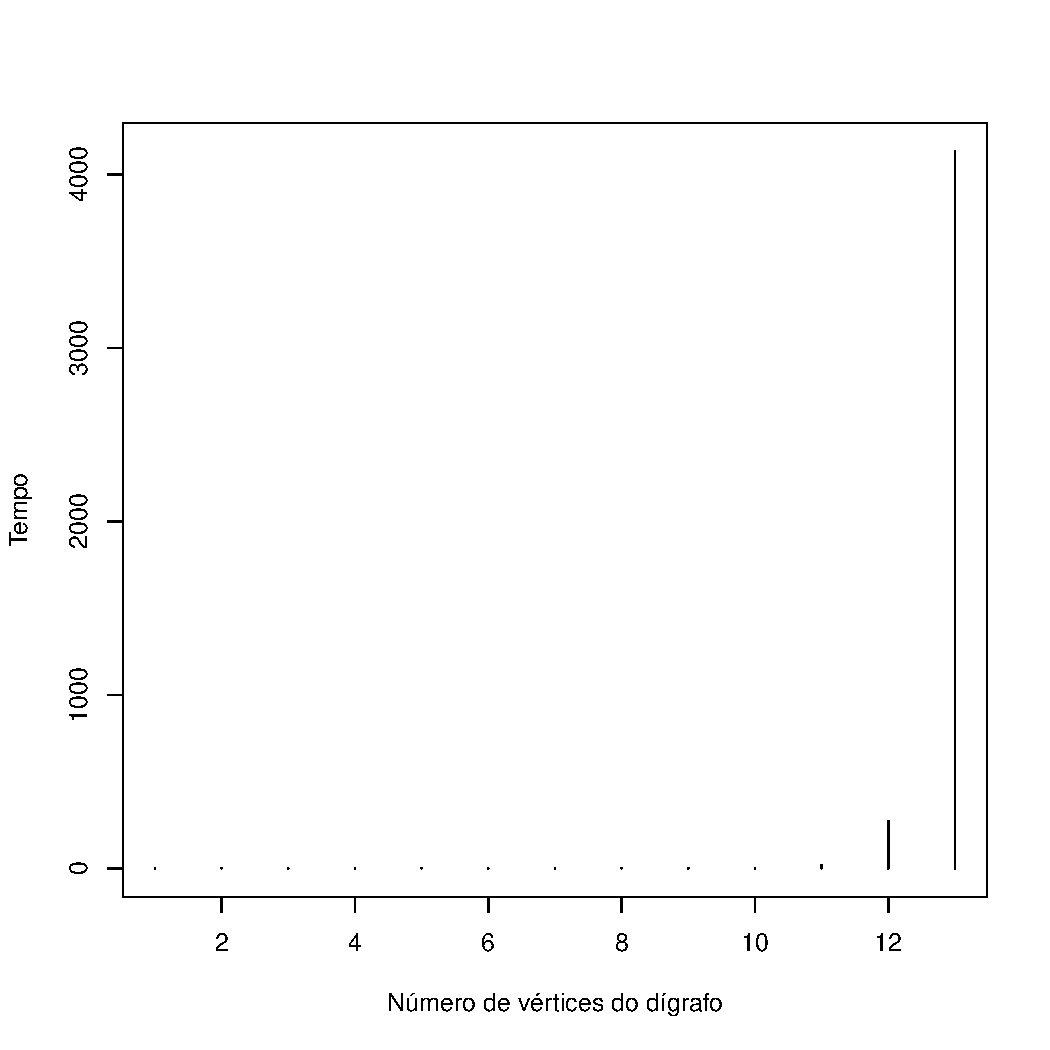
\includegraphics[scale=0.75]{sequencial.pdf}
      \caption{Tempo de execução do programa sequencial em função do número de
        vértices do dígrafo. (Testes executados num Intel Pentium 4 com clock de
        $2167$ Mhz e $2$ GB RAM DRR-2.)}
      \label{fig-sequencial}
    \end{figure}
    
    Agora, considere o experimento de variarmos a quantidade $p$ de
    processadores executando o programa paralelo e variarmos, também, o número
    $n$ de vértices do dígrafo, obtendo tempos $t(n, p)$ em função de $n$ e $p$.
    (Claro que todos os pontos ($n$, $p$, $t(n, p)$) foram gerados sob as mesmas
    condições de hardware\footnote{Todos os pontos gerados na mesma máquina e
      com apenas um usuário logado no sistema, exceto pelo root.
      Embora seja impossível obtermos condições perfeitas de hardware, porque
      precisamos do sistema operacional para executar nosso programa e o SO
      mantém outros processos em execução, as condições sob as quais esses
      resultados foram obtidos nos fornecem uma aproximação razoável das
      condições perfeitas.} ---todos os pontos gerados na máquina
    \emph{bowmore}\footnote{Bowmore é uma servidora da arquitetura x86-64 com
      $12$ processadores, clock de $2800$ Mhz, caches L1 de $64k$ (dados) +
      $64k$ (instruções) e L2 de $512k$ e $20$ GB de RAM.}.)
    
    \begin{figure}
      \centering
      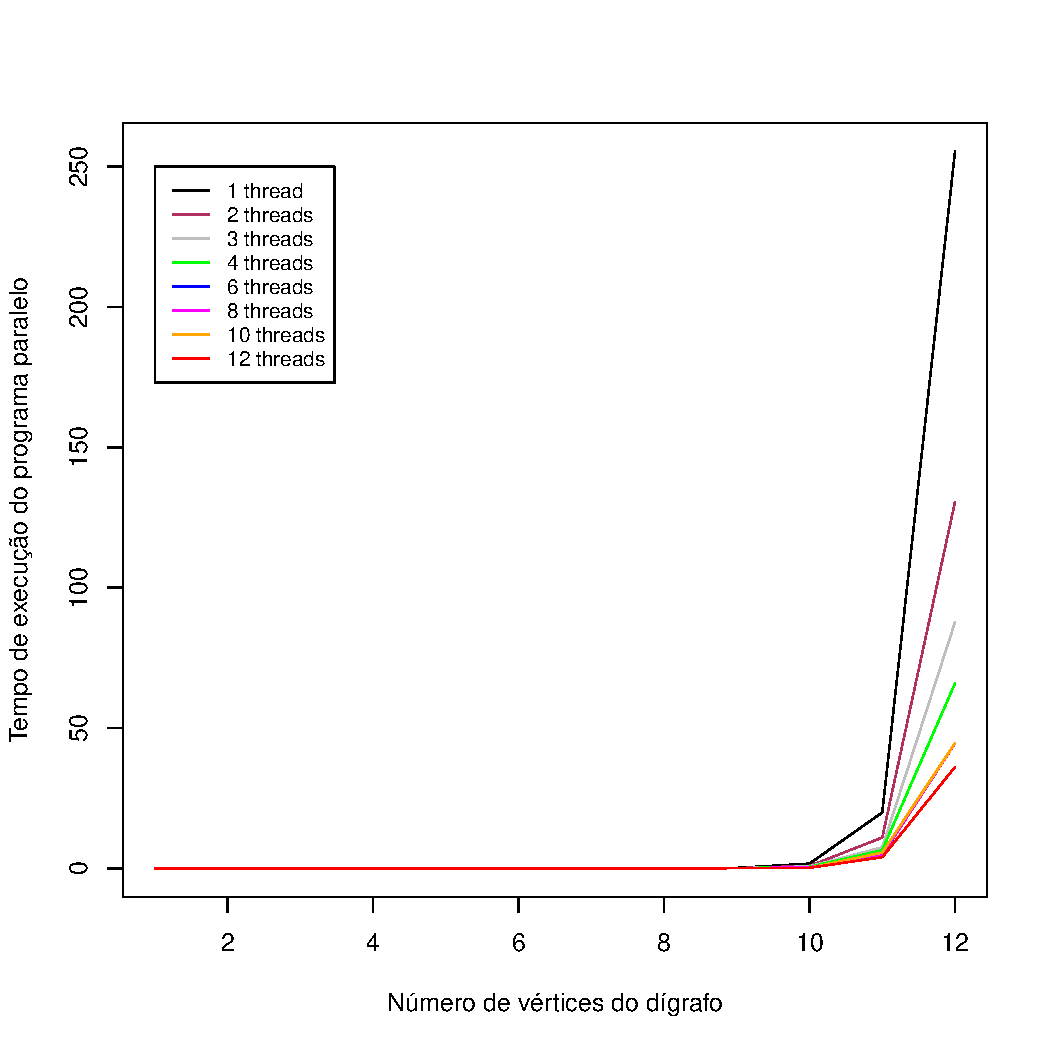
\includegraphics[scale=0.8]{paralelo.pdf}
      \caption{Tempo de execução do programa paralelo, variando o número de
        vértices do dígrafo e variando, também, o número de threads.}
      \label{fig-paralelo}
    \end{figure}

    Para mais precisão, os pontos da figura \ref{fig-paralelo} são descritos na
    seguinte tabela:

    \begin{tabular}{lrrrrrrrr}
      \toprule
      \multicolumn{8}{c}{Número de threads} \\
      \cmidrule(r){2-9}
      $n$ & 1 & 2 & 3 & 4 & 6 & 8 & 10 & 12 \\
      \midrule
      2  & 0.005 & 0.007 & 0.006 & 0.007 & 0.006 & 0.008 & 0.007 & 0.021 \\
      3  & 0.004 & 0.005 & 0.005 & 0.005 & 0.005 & 0.007 & 0.006 & 0.008 \\
      4  & 0.004 & 0.005 & 0.005 & 0.005 & 0.006 & 0.006 & 0.006 & 0.006 \\
      5  & 0.003 & 0.004 & 0.004 & 0.004 & 0.004 & 0.004 & 0.005 & 0.004 \\
      6  & 0.005 & 0.005 & 0.005 & 0.005 & 0.005 & 0.006 & 0.008 & 0.007 \\
      7  & 0.006 & 0.006 & 0.006 & 0.006 & 0.006 & 0.007 & 0.007 & 0.008 \\
      8  & 0.020 & 0.013 & 0.012 & 0.009 & 0.010 & 0.011 & 0.011 & 0.011 \\
      9  & 0.158 & 0.099 & 0.063 & 0.061 & 0.053 & 0.051 & 0.050 & 0.045 \\
      10 & 1.677 & 0.848 & 0.686 & 0.517 & 0.352 & 0.362 & 0.186 & 0.187 \\
      11 & 19.900 & 10.972 & 7.467 & 6.475 & 4.708 & 4.746 & 5.599 & 3.976 \\
      12 & 255.321 & 130.517 & 87.679 & 65.866 & 44.586 & 44.495 & 44.632 &
      36.089 \\
      \bottomrule
    \end{tabular}
    
    O compartamento dessa tabela, quando aumentamos $p$ e $n$, é conforme
    descrevemos na nossa análise, na seção anterior.

    Ajustando a função $t_P(X)$, da classe assintótica mais justa, temos um
    ajuste ótimo ao tempo empírico $t(n, p)$, ajustando apenas a constante da
    classe assintótica ---dependente única e exclusivamente do
    \emph{hardware}--- e o parâmetro da distribuição Poisson ---esse é o
    parâmetro que está correlacionado com os pontos não-decrescentes, para uma
    instância fixa e variando $p$, da tabela: a concorrência entre os
    processadores em gravar um caminho numa mesma célula causa com que apenas um
    deles tenha acesso à celula enquanto os demais aguardam, de forma
    sequencial, pelo acesso à referida célula. (Isso também é melhor discutido
    na análise da seção anterior.)

  \section{Considerações finais e conclusão}

    Visto que os limites de tempo de computação mono-core está muito próximo das
    máquinas atuais e em se tratando de um problema muito difícil de ser
    resolvido, em termos de recursos computacionais (não de programação!), não
    vemos outra alternativa para ganho de performance a não ser via
    paralelização do algoritmo sequencial.

    Os resultados obtidos foram muito atraentes, se aproximando muito do limite
    teórico. Um ajuste\footnote{É um ajuste da função
      $\textsc{tempo-relativo}(x) = 1/x$ com deslocamento, $a$, no eixo das
      abcissas  e com direito a um coeficiente, $b$, em $1/x$.} dos parâmetros
    $a$ e $b$ para o modelo
    \begin{equation*}
      \textsc{tempo-relativo}(p) = a + b/p
    \end{equation*}
    nos dá, com $95\%$ de confiança, os intervalos
    \begin{align*}
      -0.1465 \leq &a \leq -0.07484 \\
      &\e \\
      1.013 \leq &b \leq 1.179,
    \end{align*}
    fornecendo-nos $-0.1107$ e $1.096$ como melhores candidatos a $a$ e $b$,
    respectivamente.
    Então, podemos estimar o tempo de computação do programa paralelo
    (lembrando: com base na nossa tabela de tempos de execução do programa
    paralelo):
    \begin{equation*}
      t(n, p) \approx t(n, 1) \,\textsc{tempo-relativo}(p),
    \end{equation*}
    que vem novamente de encontro com a nossa análise na segunda seção, para
    alguns\footnote{Isso é uma aproximação, no intuito de facilitar a
      visualização do ganho de performance do algoritmo paralelo sobre o
      algoritmo sequencial.} valores de $p$.
    Veja os tempos de execução normalizados e o ajuste à função
    $\textsc{tempo-relativo}(p)$ na figura \ref{fig-ajuste}.

    \begin{figure}
      \centering
      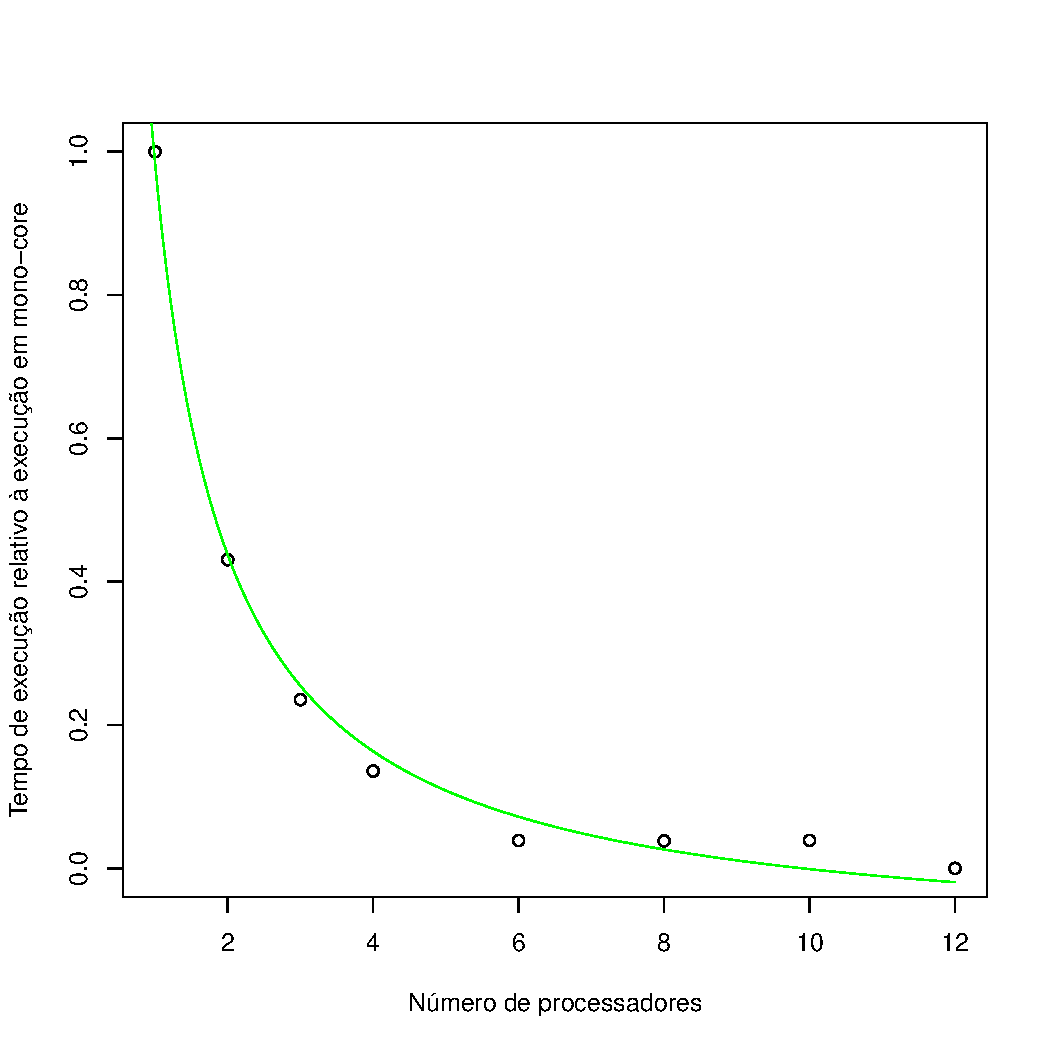
\includegraphics[scale=0.8]{ajuste.pdf}
      \caption{Tempos relativos ao número de threads e o ajuste desses tempos
        pelo modelo $\textsc{tempo-relativo}(p)$.}
      \label{fig-ajuste}
    \end{figure}

    Poderíamos estimar o ganho de performance em função do número de
    processadores sob a ótica da lei de Gustafson tomando $1 /
    \textsc{tempo-relativo}(p)$ como estimativa, em função de $p$.
    O problema é que temos um limite teórico,
    conforme explanamos\footnote{Voltamos a enfatizar que a análise mais
      rigorosa desse problema está na segunda seção.} na segunda seção, para
    esse ganho; isso confirma a lei de Amdahl, que reitera o argumento de que o
    ganho máximo, em função de $p$, é limitado.
    (Isso é decorrente da natureza do nosso problema, não porque as leis
    supracitadas se contradizem.)

  \pagebreak
  \bibliographystyle{plainnat}
  \bibliography{referencias}
    
\end{document}
